\documentclass[10pt,landscape]{article}
\usepackage{multicol}
\usepackage{calc}
\usepackage{ifthen}
\usepackage{amsmath}
\usepackage{tikz}
\usepackage[landscape]{geometry}
\usepackage{hyperref}
\usepackage{caption}
\captionsetup{
   font=small,
   labelfont=bf,
   tableposition=top
}
\usetikzlibrary{decorations.markings}
\tikzset{
    set arrow inside/.code={\pgfqkeys{/tikz/arrow inside}{#1}},
    set arrow inside={end/.initial=>, opt/.initial=},
    /pgf/decoration/Mark/.style={
        mark/.expanded=at position #1 with
        {
            \noexpand\arrow[\pgfkeysvalueof{/tikz/arrow inside/opt}]{\pgfkeysvalueof{/tikz/arrow inside/end}}
        }
    },
    arrow inside/.style 2 args={
        set arrow inside={#1},
        postaction={
            decorate,decoration={
                markings,Mark/.list={#2}
            }
        }
    },
}


% To make this come out properly in landscape mode, do one of the following
% 1.
%  pdflatex latexsheet.tex
%
% 2.
%  latex latexsheet.tex
%  dvips -P pdf  -t landscape latexsheet.dvi
%  ps2pdf latexsheet.ps


% If you're reading this, be prepared for confusion.  Making this was
% a learning experience for me, and it shows.  Much of the placement
% was hacked in; if you make it better, let me know...


% 2008-04
% Changed page margin code to use the geometry package. Also added code for
% conditional page margins, depending on paper size. Thanks to Uwe Ziegenhagen
% for the suggestions.

% 2006-08
% Made changes based on suggestions from Gene Cooperman. <gene at ccs.neu.edu>


% To Do:
% \listoffigures \listoftables
% \setcounter{secnumdepth}{0}


% This sets page margins to .5 inch if using letter paper, and to 1cm
% if using A4 paper. (This probably isn't strictly necessary.)
% If using another size paper, use default 1cm margins.
\ifthenelse{\lengthtest { \paperwidth = 11in}}
	{ \geometry{top=.5in,left=.5in,right=.5in,bottom=.5in} }
	{\ifthenelse{ \lengthtest{ \paperwidth = 297mm}}
		{\geometry{top=1cm,left=1cm,right=1cm,bottom=1cm} }
		{\geometry{top=1cm,left=1cm,right=1cm,bottom=1cm} }
	}

% Turn off header and footer
\pagestyle{empty}
 

% Redefine section commands to use less space
\makeatletter
\renewcommand{\section}{\@startsection{section}{1}{0mm}%
                                {-1ex plus -.5ex minus -.2ex}%
                                {0.5ex plus .2ex}%x
                                {\normalfont\large\bfseries}}
\renewcommand{\subsection}{\@startsection{subsection}{2}{0mm}%
                                {-1explus -.5ex minus -.2ex}%
                                {0.5ex plus .2ex}%
                                {\normalfont\normalsize\bfseries}}
\renewcommand{\subsubsection}{\@startsection{subsubsection}{3}{0mm}%
                                {-1ex plus -.5ex minus -.2ex}%
                                {1ex plus .2ex}%
                                {\normalfont\small\bfseries}}
\makeatother

% Define BibTeX command
\def\BibTeX{{\rm B\kern-.05em{\sc i\kern-.025em b}\kern-.08em
    T\kern-.1667em\lower.7ex\hbox{E}\kern-.125emX}}

% Don't print section numbers
\setcounter{secnumdepth}{0}


\setlength{\parindent}{0pt}
\setlength{\parskip}{0pt plus 0.5ex}


% -----------------------------------------------------------------------

\begin{document}

\raggedright
\footnotesize
\begin{multicols}{3}


% multicol parameters
% These lengths are set only within the two main columns
%\setlength{\columnseprule}{0.25pt}
\setlength{\premulticols}{1pt}
\setlength{\postmulticols}{1pt}
\setlength{\multicolsep}{1pt}
\setlength{\columnsep}{2pt}

\begin{center}
     \Large{Hamiltonian Mechanics Cheat Sheet} \\
\end{center}

\section{Lagrangian Mechanics}
The lagrangian of a system is a function of the coordinates $\mathbf{q}(t)$, the velocities $\mathbf{\dot q}(t)$, and time.
\begin{equation}
	L = T-V 
\end{equation}

The action of a system is the time integral of the lagrangian:
\begin{equation}
	S = \int L(\mathbf{ q}(t), \mathbf {\dot q}(t), t) dt
\end{equation}

By varying the action, and finding a stable point, we get the Euler-Lagrange equations:
\begin{equation}
	\delta S = 0 = \int \left(\frac{\partial L}{\partial \mathbf{q}}\delta \mathbf{q} + \frac{\partial L}{\partial \mathbf{\dot q}} \delta \mathbf{\dot q}\right)dt = \int \left(\frac{\partial L}{\partial \mathbf{q}}-\frac{d}{dt} \frac{\partial L}{\partial \mathbf{\dot q}} \right)\delta \mathbf{q} dt
\end{equation}
And we get the Euler-Lagrange equations:
\begin{equation}
	\frac{\partial L}{\partial \mathbf{q}}=\frac{d}{dt}\frac{\partial L}{\partial \mathbf{\dot q}}
\end{equation}

The Euler-Lagrange equations are invariant under a change of the Lagrangian by a total time derivative:
\begin{equation}
	L \rightarrow L' = L + \frac{dF}{dt}
\end{equation}
By considering a point transformation to new coordinates $Q, \dot Q$: $Q(q, t), \dot Q(q, \dot q, t) $:
\begin{equation}
	\frac{\partial \dot q}{\partial \dot Q} = \frac{\partial q}{\partial Q}
\end{equation}
Cancellation of dots.
\section{Generalised Momenta}
The Legendre transform conjugate to the velocities $\mathbf{\dot q}$ are the generalised momenta $\mathbf{p}$:
\begin{equation}
	\frac{\partial L}{\partial \mathbf{\dot q}} = \mathbf {p}
\end{equation}
If the Lagrangian is independent of a coordinate $q$, then this is called a cyclic coordinate, and the generalised momentum is conserved:
\begin{equation}
	\frac{\partial L}{\partial q} = \frac{d}{dt}\frac{\partial L}{\partial \dot q} = \dot p = 0
\end{equation}
\section{Noether's Theorem}
If the Euler-Lagrange equations are invariant under some infinitesimal coordinate transform $\mathbf {q} \rightarrow \mathbf {q} + \epsilon \mathbf {w}(s_1, \mathellipsis, s_n, \mathbf{q}, t)$, then this transform changes the Lagrangian by a total time derivative. We can taylor expand in the infinitesimal $\epsilon$ to give:
\begin{equation}
	L - \epsilon \frac{dG}{dt} = L + \epsilon\left(\frac{\partial L}{\partial \mathbf{q}}\cdot\mathbf{w} + \frac{\partial L}{\partial \mathbf{\dot q}}\cdot\mathbf{\dot w}\right) = L + \epsilon\frac{d}{dt}\left(\frac{\partial L}{\partial \mathbf{\dot q}}\cdot\mathbf{w}\right)
\end{equation}
Which implies:
\begin{equation}
	I = G + \frac{\partial L}{\partial \mathbf{\dot q}}\cdot \mathbf{w} = \mathrm{constant}
\end{equation}
\section{The Hamiltonian}
The Hamiltonian is the Legendre transform of the Lagrangian with respect to the velocity.
\begin{equation}
	H(\mathbf{q}, \mathbf{p}, t) = \frac{\partial L}{\partial \mathbf{\dot q}}\cdot \mathbf{\dot q} - L
\end{equation}

We can get Hamilton's equations by considering the differential of H:
\begin{equation}
	dH = \frac{\partial H}{\partial \mathbf{q}}\cdot d\mathbf{q} + \frac{\partial H}{\partial \mathbf{p}}\cdot d\mathbf{p} + \frac{\partial H}{\partial t}
\end{equation}
\begin{equation}
	dH = \mathbf{\dot q} \cdot d\mathbf{p} - \mathbf{\dot p} \cdot d\mathbf{q} - \frac{\partial L}{\partial t}
\end{equation}
Equating the coefficients of the differentials, we get Hamilton's equations of motion:
\begin{equation}
	\mathbf v =
	\frac{d}{dt}
	\begin{pmatrix}
		\mathbf{q} \\
		\mathbf{p}
		\end{pmatrix} = 
		\begin{pmatrix}
			\nabla_\mathbf{p}H \\ 
		-\nabla_\mathbf{q}H
		\end{pmatrix}\mathrm{\ \ \ and\ \ \ } \frac{\partial H}{\partial t} = -\frac{\partial L}{\partial t}
\end{equation}

Where $\mathbf v$ is the phase space velocity. If the Hamiltonian is time-independent, then the motion in phase space lies along paths of constant energy:
\begin{equation}
	\mathbf {v}\cdot \nabla H = \nabla_\mathbf{p}H\cdot\nabla_\mathbf{q} H - \nabla_\mathbf{q}H\cdot\nabla_\mathbf{p} H = 0
\end{equation}
\section{Liouville's Theorem}

The ``fluid'' system is incompressible in phase space, and if the Hamiltonian is independent of time then the phase space fluid is constant.

Incompressibility is shown by:
\begin{equation}
	\nabla \cdot\mathbf{v} = \nabla_\mathbf{q}\cdot\nabla_\mathbf{p}H - \nabla_\mathbf{p}\cdot\nabla_\mathbf{q} H = 0
\end{equation}
The density $\rho$ obeys the equation:
\begin{equation}
	\frac{d\rho}{dt} = \frac{\partial \rho}{\partial t} + \nabla \cdot (\rho \mathbf{v}) = 0
\end{equation}
The virial theorem tells us that when averaged over time:
\begin{equation}
	\overline{\mathbf{p}\cdot\frac{\partial H}{\partial \mathbf{p}}} = \overline{\mathbf{q}\cdot \frac{\partial H}{\partial \mathbf{q}}}
\end{equation}
\section{Qualitative Dynamics}
Have systems described by a velocity $\mathbf {\dot r}$. These systems have fixed points at $\mathbf{\dot r}=\mathbf {0}$, which we call $\mathbf{r^*}$.

We can expand linearly around these fixed points to find the behaviour of the system:
\begin{equation}
\dot r^i(\mathbf{r^*}+\delta\mathbf{r}) \approx \dot r^i(\mathbf{r^*}) + \left.\frac{\partial \dot r^i}{\partial x^j}\right|_{\mathbf{r^*}} \delta r^j = A^i_j \delta r^j 
\end{equation}
Where $x^i$ are the coordinates, and the matrix $A^i_j$ is the jacobian of the velocity vector.

We can then look for solutions of $\delta \mathbf{\dot r}(t)=\mathbf{A}\delta\mathbf{r}$:
\begin{equation}
	\lambda we^{\lambda t} = \mathbf{A}\mathbf{w}e^{\mathbf{A}t}
\end{equation}
And we have an eigenvalue equation:
\begin{equation}
	\det{(\mathbf{A}-\lambda\mathbf{I})} = 0
\end{equation}
And can work out the eigenvectors:
\begin{equation}
	(\mathbf{A}-\lambda_i\mathbf{I})\mathbf{w}_i = 0
\end{equation}
\subsection{Eigenvalue Behaviours}
The behaviour of 2D systems for a range of eigenvalues is illstrated next.

For real and distinct eigenvalues, $\lambda_1\neq\lambda_2\neq0$, the system has the behaviours:
\begin{center}
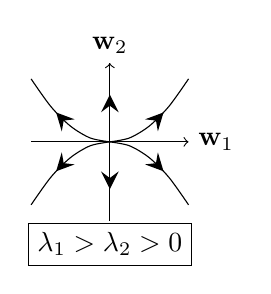
\begin{tikzpicture}
    \draw[->] (-1,0) -- (1,0) node[right] {$\mathbf{w}_1$};
     \draw[->] (0,-1) -- (0,1) node[above] {$\mathbf{w}_2$};
	%\draw[smooth, samples=100, domain=0:1] plot({\x*cos(360*\x)}, {\x*sin(360*\x)});
      \draw[smooth, samples=5, domain=0:1] plot({\x)}, {0.8*\x*\x)}) [arrow inside={end=stealth,opt={scale=2}}{0.6}];
      \draw[smooth, samples=5, domain=0:1] plot({-\x)}, {0.8*\x*\x)}) [arrow inside={end=stealth,opt={scale=2}}{0.6}];
      \draw[smooth, samples=5, domain=0:1] plot({\x)}, {-0.8*\x*\x)}) [arrow inside={end=stealth,opt={scale=2}}{0.6}];
      \draw[smooth, samples=5, domain=0:1] plot({-\x)}, {-0.8*\x*\x)}) [arrow inside={end=stealth,opt={scale=2}}{0.6}];
      \draw[smooth, samples=5, domain=0:1] plot(0, \x) [arrow inside={end=stealth,opt={scale=2}}{0.6}];
      \draw[smooth, samples=5, domain=0:1] plot(0, -\x) [arrow inside={end=stealth,opt={scale=2}}{0.6}];
	\node[draw] at (0, -1.3) {$\lambda_1>\lambda_2>0$};
\end{tikzpicture}
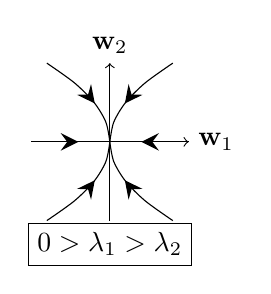
\begin{tikzpicture}
    \draw[->] (-1,0) -- (1,0) node[right] {$\mathbf{w}_1$};
     \draw[->] (0,-1) -- (0,1) node[above] {$\mathbf{w}_2$};
	%\draw[smooth, samples=100, domain=0:1] plot({\x*cos(360*\x)}, {\x*sin(360*\x)});
     \draw[smooth, samples=5, domain=1:0] plot({0.8*\x*\x}, {\x}) [arrow inside={end=stealth,opt={scale=2}}{0.6}];
      \draw[smooth, samples=5, domain=1:0] plot({0.8*\x*\x}, {-\x}) [arrow inside={end=stealth,opt={scale=2}}{0.6}];
      \draw[smooth, samples=5, domain=1:0] plot({-0.8*\x*\x}, {\x}) [arrow inside={end=stealth,opt={scale=2}}{0.6}];
      \draw[smooth, samples=5, domain=1:0] plot({-0.8*\x*\x}, {-\x}) [arrow inside={end=stealth,opt={scale=2}}{0.6}];
      \draw[smooth, samples=5, domain=1:0] plot(\x, 0) [arrow inside={end=stealth,opt={scale=2}}{0.6}];
      \draw[smooth, samples=5, domain=1:0] plot(-\x, 0) [arrow inside={end=stealth,opt={scale=2}}{0.6}];
	\node[draw] at (0, -1.3) {$0>\lambda_1>\lambda_2$};
\end{tikzpicture}
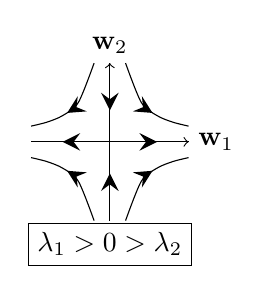
\begin{tikzpicture}
    \draw[->] (-1,0) -- (1,0) node[right] {$\mathbf{w}_1$};
     \draw[->] (0,-1) -- (0,1) node[above] {$\mathbf{w}_2$};
	%\draw[smooth, samples=100, domain=0:1] plot({\x*cos(360*\x)}, {\x*sin(360*\x)});
     \draw[smooth, samples=5, domain=0.2:1] plot({\x)}, {1/(5*\x)}) [arrow inside={end=stealth,opt={scale=2}}{0.6}];
     \draw[smooth, samples=5, domain=0.2:1] plot({-\x)}, {1/(5*\x)}) [arrow inside={end=stealth,opt={scale=2}}{0.6}];
     \draw[smooth, samples=5, domain=0.2:1] plot({\x)}, {-1/(5*\x)}) [arrow inside={end=stealth,opt={scale=2}}{0.6}];
     \draw[smooth, samples=5, domain=0.2:1] plot({-\x)}, {-1/(5*\x)}) [arrow inside={end=stealth,opt={scale=2}}{0.6}];
      \draw[smooth, samples=5, domain=0:1] plot(\x, 0) [arrow inside={end=stealth,opt={scale=2}}{0.6}];
      \draw[smooth, samples=5, domain=0:1] plot(-\x, 0) [arrow inside={end=stealth,opt={scale=2}}{0.6}];
      \draw[smooth, samples=5, domain=1:0] plot(0, \x) [arrow inside={end=stealth,opt={scale=2}}{0.6}];
      \draw[smooth, samples=5, domain=1:0] plot(0, -\x) [arrow inside={end=stealth,opt={scale=2}}{0.6}];
	\node[draw] at (0, -1.3) {$\lambda_1>0>\lambda_2$};
\end{tikzpicture}
\end{center}
An unstable repeller, a stable attractor and an unstable saddle point.

For real degenerate eigenvalues, $\lambda_1=\lambda_2\neq0$:
\begin{center}
	\begin{tikzpicture}
    \draw[->] (-1,0) -- (1,0) node[right] {$\mathbf{w}_1$};
     \draw[->] (0,-1) -- (0,1) node[above] {$\mathbf{w}_2$};
	%\draw[smooth, samples=100, domain=0:1] plot({\x*cos(360*\x)}, {\x*sin(360*\x)});
     \draw[smooth, samples=2, domain=0:1] plot({\x}, {\x}) [arrow inside={end=stealth,opt={scale=2}}{0.6}];
     \draw[smooth, samples=2, domain=0:1] plot({\x}, {0}) [arrow inside={end=stealth,opt={scale=2}}{0.6}];
     \draw[smooth, samples=2, domain=0:1] plot({\x}, -{\x}) [arrow inside={end=stealth,opt={scale=2}}{0.6}];
     \draw[smooth, samples=2, domain=0:1] plot({0}, {\x}) [arrow inside={end=stealth,opt={scale=2}}{0.6}];
     \draw[smooth, samples=2, domain=0:1] plot({0}, {-\x}) [arrow inside={end=stealth,opt={scale=2}}{0.6}];
     \draw[smooth, samples=2, domain=0:1] plot({-\x}, {\x}) [arrow inside={end=stealth,opt={scale=2}}{0.6}];
     \draw[smooth, samples=2, domain=0:1] plot({-\x}, {0}) [arrow inside={end=stealth,opt={scale=2}}{0.6}];
     \draw[smooth, samples=2, domain=0:1] plot({-\x}, -{\x}) [arrow inside={end=stealth,opt={scale=2}}{0.6}];
	\node[draw] at (0, -1.3) {$\lambda_1=\lambda_2>0$};
	\end{tikzpicture}
	\begin{tikzpicture}
    \draw[->] (-1,0) -- (1,0) node[right] {$\mathbf{w}_1$};
     \draw[->] (0,-1) -- (0,1) node[above] {$\mathbf{w}_2$};
	%\draw[smooth, samples=100, domain=0:1] plot({\x*cos(360*\x)}, {\x*sin(360*\x)});
     \draw[smooth, samples=2, domain=1:0] plot({\x}, {\x}) [arrow inside={end=stealth,opt={scale=2}}{0.6}];
     \draw[smooth, samples=2, domain=1:0] plot({\x}, {0}) [arrow inside={end=stealth,opt={scale=2}}{0.6}];
     \draw[smooth, samples=2, domain=1:0] plot({\x}, -{\x}) [arrow inside={end=stealth,opt={scale=2}}{0.6}];
     \draw[smooth, samples=2, domain=1:0] plot({0}, {\x}) [arrow inside={end=stealth,opt={scale=2}}{0.6}];
     \draw[smooth, samples=2, domain=1:0] plot({0}, {-\x}) [arrow inside={end=stealth,opt={scale=2}}{0.6}];
     \draw[smooth, samples=2, domain=1:0] plot({-\x}, {\x}) [arrow inside={end=stealth,opt={scale=2}}{0.6}];
     \draw[smooth, samples=2, domain=1:0] plot({-\x}, {0}) [arrow inside={end=stealth,opt={scale=2}}{0.6}];
     \draw[smooth, samples=2, domain=1:0] plot({-\x}, -{\x}) [arrow inside={end=stealth,opt={scale=2}}{0.6}];
	\node[draw] at (0, -1.3) {$0>\lambda_1=\lambda_2$};
	\end{tikzpicture}
\end{center}
An unstable repeller and a fixed attractor.

For $\mathbf{A}=\begin{pmatrix}\alpha & -\omega \\ \omega & \alpha\end{pmatrix}$, we have complex eigenvalues $\lambda_{\pm}=\alpha\pm i\omega$, which cause rotations.
It is easier to think polar coordinates in this case, with $\delta \dot r = \alpha \delta r$ and $\dot \theta = \omega$.
There are 3 types of fixed point in this case:
\begin{center}
	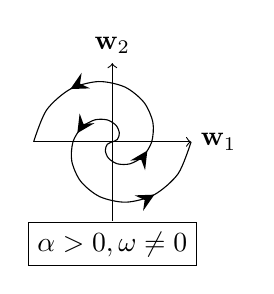
\begin{tikzpicture}
    \draw[->] (-1,0) -- (1,0) node[right] {$\mathbf{w}_1$};
     \draw[->] (0,-1) -- (0,1) node[above] {$\mathbf{w}_2$};
	\draw[smooth, samples=15, domain=0:1] plot({\x*cos(360*\x)}, {\x*sin(360*\x)}) [arrow inside={end=stealth,opt={scale=2}}{0.25, 0.75}];
	\draw[smooth, samples=15, domain=0:1] plot({-\x*cos(360*\x)}, {-\x*sin(360*\x)}) [arrow inside={end=stealth,opt={scale=2}}{0.25, 0.75}];
     \node[draw] at (0, -1.3) {$\alpha>0, \omega\neq0$};
	\end{tikzpicture}
	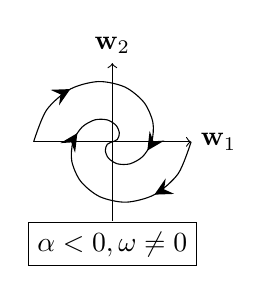
\begin{tikzpicture}
    \draw[->] (-1,0) -- (1,0) node[right] {$\mathbf{w}_1$};
     \draw[->] (0,-1) -- (0,1) node[above] {$\mathbf{w}_2$};
	\draw[smooth, samples=15, domain=1:0] plot({\x*cos(360*\x)}, {\x*sin(360*\x)}) [arrow inside={end=stealth,opt={scale=2}}{0.25, 0.75}];
	\draw[smooth, samples=15, domain=1:0] plot({-\x*cos(360*\x)}, {-\x*sin(360*\x)}) [arrow inside={end=stealth,opt={scale=2}}{0.25, 0.75}];
     \node[draw] at (0, -1.3) {$\alpha<0, \omega\neq0$};
	\end{tikzpicture}
	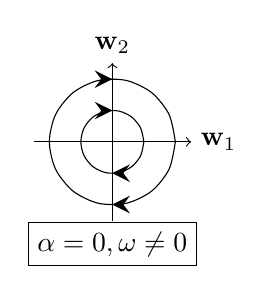
\begin{tikzpicture}
    \draw[->] (-1,0) -- (1,0) node[right] {$\mathbf{w}_1$};
     \draw[->] (0,-1) -- (0,1) node[above] {$\mathbf{w}_2$};
     \draw[smooth, samples=15, domain=1:0] plot({0.8*cos(360*\x)}, {0.8*sin(360*\x)}) [arrow inside={end=stealth,opt={scale=2}}{0.25, 0.75}];
	\draw[smooth, samples=15, domain=1:0] plot({0.4*cos(360*\x)}, {0.4*sin(360*\x)}) [arrow inside={end=stealth,opt={scale=2}}{0.25, 0.75}];
     \node[draw] at (0, -1.3) {$\alpha=0, \omega\neq0$};
	\end{tikzpicture}
\end{center}
\end{document}
\end{verbatim}

\rule{0.3\linewidth}{0.25pt}
\scriptsize


\end{multicols}
\end{document}
